\newcommand{\todo}[1]{{\bf TODO} #1}
\newif\ifPAPER  
%\PAPERtrue % select either slide or note
\PAPERfalse  

\def\t{\title{INCL intra-nuclear cascade development in C++ for Geant4}}

\def\a{
\author{P.~Kaitaniemi}
\affiliation{CEA/Saclay}
}

\newcommand{\codeAlgorithm}[1]{
\addcontentsline{toc}{section}{Résumé}
\begin{center}\fbox{\parbox{12cm}{\bf #1}}\end{center}}

\newcommand{\cppintro}[1]{
\lstset{language=C,
caption= #1 ,
label=listing:boundary}}

\def\cppstart{\begin{lstlisting}}
\def\cppend{\end{lstlisting}}

\newif\ifCITENOTE 
\CITENOTEtrue

\ifPAPER

\else   % Slides ---------------------------------------------------------------

\documentclass[slidestop,compress,xdvips,10pt]{beamer} 
\usetheme{Antibes}
\usecolortheme{lily}
\usepackage{graphicx}
\usepackage{hyperref}
\usepackage{listings}
\usepackage{verbatim} % for comment
\transglitter[direction=315]
\xdefinecolor{ahcol}{rgb}{0.2, 0.4, 0.1}
\xdefinecolor{olive}{cmyk}{0.64,0,0.95,0.4}
\colorlet{structure}{green!60!black} % for color substitution
\usepackage{color} % for definecolor
\definecolor{light-gray}{gray}{0.95}
\definecolor{dark-gray}{gray}{0.30}
\definecolor{orange}{rgb}{1,0.5,0}
\definecolor{dark-blue}{cmyk}{1,0.5,0.5,0}
\usepackage{attachfile} 
\hypersetup{
    a4paper, % page format
    pdftitle={My Title},                  % Title
    pdfsubject={Subject of the document}, % Subject 
    pdfauthor={Author name},              % Author
    pdfkeywords={list of keywords},       % Keywords
    plainpages=true, %
    colorlinks,       % links are colored
    urlcolor=dark-blue,    % color of external links
    linkcolor=dark-blue,    % color of internal links
    citecolor=black,  % color of links to bibliography
    bookmarksnumbered
}

\usecolortheme[named=ahcol]{structure}
\useoutertheme{myinfolines}
\useinnertheme{rounded}
\setbeamercolor{alerted_text}{fg=blue}

\makeatother
\beamertemplatetransparentcoveredhigh
\t
\author{Pekka Kaitaniemi\footnote{pekka.kaitaniemi@cea.fr} \\
\vskip1.0cm
CEA/Saclay, SPhN \\
Helsinki Institute of Physics \\
Geant4 Collaboration}

\graphicspath{{.}{figures/}}
\graphicspath{{images/}}
\begin{document}

\frame{\titlepage}

\section{}
\subsection{}
\frame{
\frametitle{INCL, Liege intra-nuclear cascade}
\begin{minipage}{1.0\textwidth}
\begin{minipage}{0.5\textwidth}
\begin{table}
\begin{tabular}{|l|l|}
Projectile & $p$, $n$, $\pi$ \\
           & deuteron, triton, He3, alpha \\
Energy range & 150 MeV - 3 GeV \\
Target nuclei & Carbon - Uranium
\end{tabular}
\caption{INCL \footnote{A. Boudard, C. Volant, S. Leray, J.C. David (CEA/SPhN),
J. Cugnon, T. Aoust, P. Henrotte (Univ. Li\'{e}ge - Belgium)} key features}
\end{table}
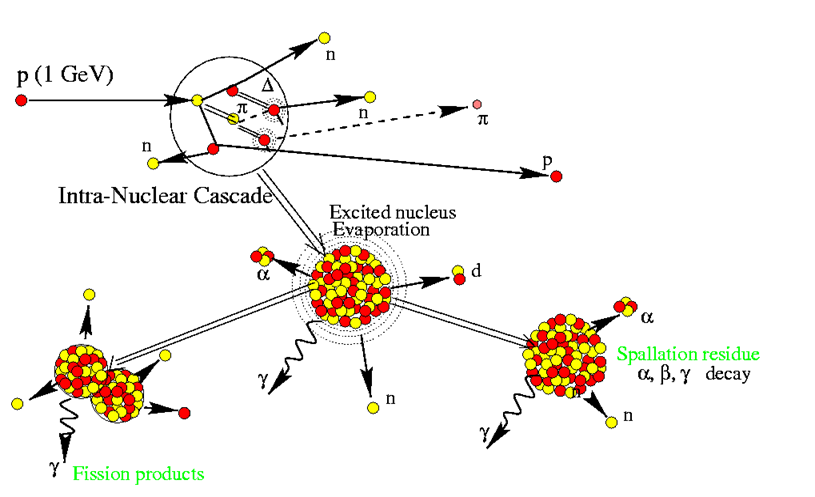
\includegraphics[width=1.0\textwidth]{inclSchematic}
\end{minipage}
\begin{minipage}{0.5\textwidth}
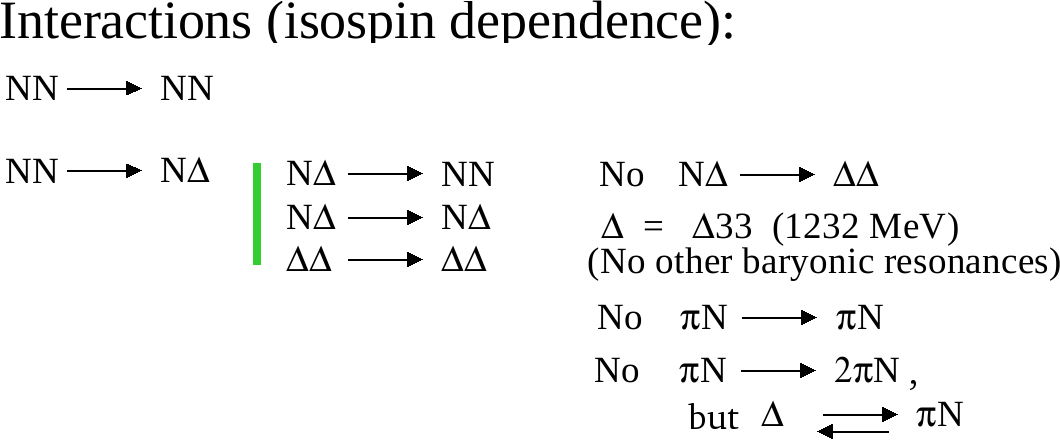
\includegraphics[width=1.0\textwidth]{interactions}
\end{minipage}
\end{minipage}
}

\subsection{}
\frame{
\frametitle{INCL4.3}
INCL\footnote{A. Boudard, C. Volant, S. Leray, J.C. David (CEA/SPhN),
J. Cugnon, T. Aoust, P. Henrotte (Univ. Li\'{e}ge - Belgium)} provides spallation model
coupled with evaporation and fission models.
\vspace{0.4cm}

\begin{itemize}
\item Possibility to use Geant4 Fermi break-up or
ABLA\footnote{K-H Schmidt, A. Kelic, J. Benlliure GSI and Univ Santiago de C.} 
de-excitation (evaporation and fission).

\item Based on physics (phenomenology reduced)
to be predictive.

\item $\sigma(E)$ and $d\sigma/d\Sigma(\theta)$ from experiments,
no ad hoc parameters in the model.

\item Series of elementary scattering explicitly followed in time.

\item Trajectories are straight lines.
\end{itemize}
%REMINDER: There is no $\pi N \rightarrow \pi N$, but it is partly taken
%          into account through $\Delta$ formation and decay.
\begin{center}
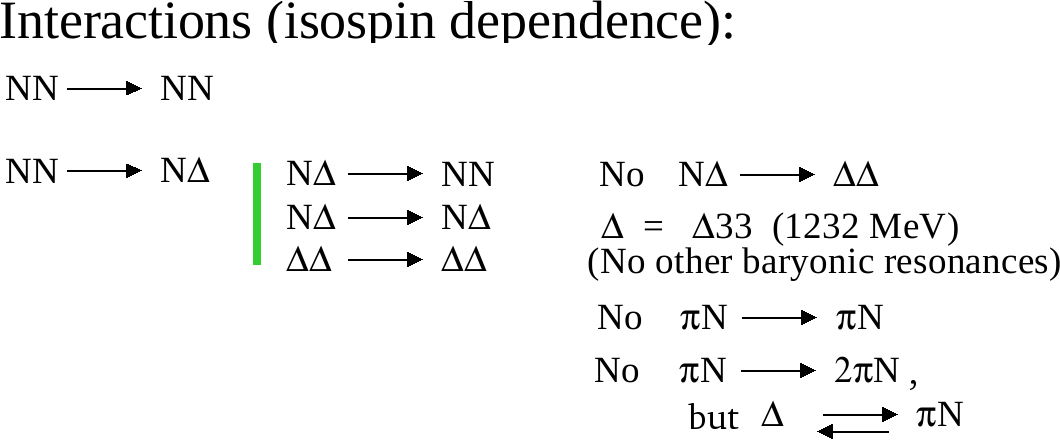
\includegraphics[width=0.6\textwidth]{interactions}
\end{center}
% No piN->piN  but piN<->Delta  
% NOTE: Say that there is no explicit piN scattering but through a 
%       \Delta formation and decay it is partly taken into account.
}

\subsection{}
\frame{
\frametitle{INCL4.3 (cont.)}
\begin{itemize}
\item Pauli blocking on nucleons after each events + long range correlation (CDPP).

\item No collision between spectators, only reflections (cannot escape).

\item Stopping time of the cascade:   $t_{max}= 70.0~\mathrm{fm/c}~(A/208)^{0.16}$.

\item Current version INCL4.3. supports
light cluster production (d, t, $^3$He, $^4$He)\footnote{First version 
       of light cluster production Nucl. Phys. A740 (2004) 195}.

\item All outgoing particles (remnant nucleus, nucleons, pions)
characterised by (A, Z, E$^{*}$, J, P, $\theta$, $\phi$).
\end{itemize}
}

\end{document}

\fi %slides



